% !TeX encoding = UTF-8
% !TeX program = pdflatex
% !TeX spellcheck = it_IT

% \documentclass[a4paper, 11pt]{article}
\documentclass[Lau,binding=0.6cm]{sapthesis}

\usepackage{microtype}
\usepackage[italian]{babel}
\usepackage[utf8]{inputenx}
\usepackage[hidelinks]{hyperref}
\usepackage{amssymb}
\usepackage{hyperref}
\usepackage{rotating}

\usepackage{hypcap}
\usepackage{titlesec}
\titleformat{\chapter}[hang]{\Huge\bf}{\thechapter{. }}{0pt}{\Huge\bf}

\newcommand{\RomanNumeralCaps}[1]
    {\MakeUppercase{\romannumeral #1}}

\graphicspath{ {./images/} }

\hypersetup{pdftitle={tesi},pdfauthor={Andrei Laurentiu Lepadat}}

\title{Utilizzo di Sensor Noise Fingerprint per il Rilevamento di Cyber-Attacchi in CPS}
\author{Andrei Laurentiu Lepadat}
\IDnumber{1677093}
\course{Informatica}
\courseorganizer{Facoltà di Ingegneria dell'Informazione, Informatica e Statistica}
\AcademicYear{2020/2021}
\copyyear{2021}
\advisor{Prof. Enrico Tronci}
\authoremail{lepadat.1677093@studenti.uniroma1.it}

\versiondate{\today}

\begin{document}

\frontmatter

\maketitle

\dedication{Decidere se inserire. Ne vale la pena?}

% ----------------------------------------------------------------------------------------

\tableofcontents

\chapter{Sommario} 
% Massimo una pagina da scrivere alla fine

% ----------------------------------------------------------------------------------------   

\mainmatter

\chapter{Introduzione}
% Scrivere alla fine 

\section{Contesto}
% Short description of context,  for example:
% Tutti gli essere vivneti per sopravviver hanno bisogno di alimentarsi.
% Gli uomini sono essere viventi, e quindi hanno bisogno di alimentarsi.

\section{Motivazioni}
% Motivation for what we want to do. esempio:
% Purtroppo la mancanza di una alimentazione adeguata è uno dei problemi più importanti nei paesi sottosviluppati

\section{Contributi}
% Describe here your contributions, namely the missing items identified in the motivations. esempio:
% Questo lavoro propone un metodo per generare cibo per tutti gli abitanti dei paesi sottosviluppati ...

\section{Stato dell'arte}
% Describe here the state of the art (e.g., algorithms and tools  available).
% For each paper/tool explain what you do that is not already available (killing).

\section{Struttura}
% Give an outline of the thesis structure (one sentence per section)


% ----------------------------------------------------------------------------------------

\chapter{Background}\label{chap:1}
% Put in this section all the background knowledge needed to understand what you did.
% Parlare di dati di sensori, serie temporali estratti dai sensori, rmse, rumore intrinseco sensori --> residual
% machine learning model e decision 

Ogni sistema cyber-fisico che si rispetti è dotato di almeno un sensore che ha il compito di misurare una determinata ``qualità'' fisica di interesse per il sistema stesso. 
I dati che vengono rilevati dai sensori spesso vengono memorizzati localmente e/o in modo remoto e possono essere impiegati,
come nel lavoro qui presentato, per fini paralleli o trasversali a quelli per cui sono stati installati.
Una sequenza di dati estratti da sensori ordinata temporalmente viene chiamata \textit{serie temporale} (\textit{time-series} in inglese).

Comunemente i sensori sono imperfetti per costruzione e contengono intrinsecamente un'incertezza (\textit{rumore}) nelle misurazioni che eseguono, dovuta a imperfezioni di fabbricazione.
Sia 
\begin{equation}
\bar{y}_{k} = y_{k} + \delta_{k}\label{eq:1}
\end{equation}
il valore misurato da un determinato sensore nell'istante di tempo \textit{k}, composto da $y_k$, il valore effettivo in quell'istante della grandezza misurata, più $\delta_k$, il rumore aggiunto.

In un determinato istante di tempo, il valore di ogni sensore del sistema costituisce lo \textit{stato} del sistema.
La sfida di estrarre il fingerprint dai sensori è data dal fatto che questi stati sono dinamici. 
Prendendo in considerazione, per esempio, un termometro, se la temperatura dell'ambiente che misura rimane costante nel tempo è facile estrarre il fingerprint del rumore e costruirne il profilo, 
ma in processi reali non è così semplice, gli stati cambiano continuamente, per esempio l'aumento di velocità di una macchina per via della pressione sul pedale dell'acceleratore.
\`E importante catturare queste variazioni affinch\'e le misurazioni dinamiche dei sensori possano essere stimate.
In [1] questo problema viene affrontato definendo un modello analitico del sistema interessato, rappresentato tramite il modello \textit{State-Space}. 
Vengono implementate le tecniche definite in [2], definendo cos\`i il modello lineare tempo inviariante (LTI) del sistema, rappresentato dal sistema di equazioni
\begin{equation}\label{eq:4}
    \begin{cases}
        x_{k+1} = Ax_k + Bu_k + \vartheta_k, \\
        y_k = Cx_k + \eta_k:
    \end{cases}
\end{equation}
in cui $x_k \in \mathbb{R}^n$ rappresenta lo stato del sistema, $u_k \in \mathbb{R}^p$ l'input di controllo e
$\vartheta_k$ il rumore al tempo $k$.
$y_k \in \mathbb{R}_m$ e $\eta_k \in \mathbb{R}_m$ rappresentano, rispettivamente, la misurazione e il rumore del sensore al tempo $k$.
$A$, $B$, $C$ sono le matrici dello spazio di stato di dimensioni adeguate che rappresentato la dinamica del sistema.

Definito il precedente sistema, ci sono molti punti che un attaccante mal intenzionato potrebbe bersagliare.
Nel lavoro presentato, cos\`i come in [1], vengono presi in considerazione \textit{spoofing attack} ai sensori che potrebbero essere portati a termine tramite uno schema \textit{Man-in-The-Middle}.
L'equazione lineare che rappresenta questa tipologia di attacchi \`e data da
\begin{equation}
\bar{y}_{k} = y_{k} + \delta_{k} = Cx_k + \eta_k + \delta_k,\footnote{Notare l'ugualianza con l'equazione \ref{eq:1}: un attacco \`e considerato come un'introduzione di rumore nella misurazione fatta da un sensore.}
\end{equation}
in cui $\delta_k \in \mathbb{R}_m$ rappresenta un attacco ai sensori.

In [1], dato l'output $\bar{y}_k$, viene adoperato il \textit{filtro di Kalman} per stimare lo stato del sistema e il vettore dei \textit{residui}, definito, in questo contesto, come la differenza tra la reale misurazine effettuata dal sensore
e la stima della misurazione calcolata dal filtro nell'istante $k$:
\begin{equation}
    r_k := \bar{y}_k - \hat{y}_k,
\end{equation}
dove $\hat{y}_k$ \`e l'output del filtro di Kalman.

Detto ci\`o, per quantificare la bont\`a del modello del sistema, viene utilizzato l'\textit{Errore Quadratico Medio (RMSE)}, definito come
\begin{equation}
    RMSE = \sqrt{\frac{\sum_{i=1}^n (y_i - \hat{y}_i)^2}{n}}\label{eq:5}.
\end{equation}
Questa metrica rappresenta la distanza tra il valore stimato e quello misurato, ovvero quanto il primo \`e lontano dal secondo.
Nella letteratura della teoria del controllo, modelli con un'accuratezza\footnote{Se l'RMSE rappresenta un errore, l'accuratezza viene calcolata come 100 - RMSE.} superiore al 70\% sono considerati accettabili approssimazioni della dinamica di sistemi reali.

Per ogni momento statistico (media, deviazione standard, \ldots) di una serie storica (ma non solo) si pu\`o definire un \textit{intervallo di confidenza} 
che esprime la probabilit\`a che il valore calcolato sugli $N$ campioni della serie approssimi il valore effettivo del momento statistico.
Questo intevallo, nel caso del valore medio, si definisce come 
\begin{equation}
    Pr\{\bar{x} - \epsilon \leq \mu \leq \bar{x} + \epsilon\} = 1 - \delta,
    \label{eq:2}
\end{equation}
in cui $\mu$ e $\bar{x}$ sono, rispettivamente, la media effettiva e quella calcolata. $\epsilon$ e $\delta$ sono valori che dipendono da $N$, e mantenendo $\delta$ costante
e incrementando $N$, anche $\epsilon$ cresce, allargando l'intervallo di confidenza.
Tale intervallo pu\`o essere definito anche per momenti di ordine superiore.

Nel contesto del presente lavoro, come si vedr\`a, volendo giudicare la legittimit\`a delle misurazioni di un determinato sensore, determinate propriet\`a statistiche delle nuove misurazioni (nuove nel contesto di normale 
funzionamento del sistema \textit{aperto} ad attacchi) verranno confrontate con le stesse propriet\`a di misurazioni effettuate in condizioni \textit{sicure} (questi valori sono chiamati valori di \textit{reference}). 
Per le nuove misurazioni, prendendo ancora in esempio il valore medio e volendo avere un intervallo di confidenza il pi\`u piccolo possibile (quindi un $\epsilon$ il pi\`u piccolo possibile), bisogna essere attenti per via di valori di $N$ non molto grandi,
caratteristica preferibile in quanto non si vogliono campionare troppi valori in situazioni real-time (equivarrebbe ad aspettare di pi\`u per prendere una decisione, e quindi essere potenzialmente per più tempo sotto attacco).
Scegliere un'intervallo di condifenza delle nuove misurazioni troppo grande potrebbe portare ad una sovrapposizione tra il nuovo intervallo ed quello di reference\footnote{Il caso ideale sarebbe o di inclusione del primo nel secondo o di disgiunzione, rilevando nel primo caso un valore ammesso e nel secondo caso un attacco.}.
Per avere una sensibilit\`a migliore contro gli attacchi il problema viene affrontato avvalendosi dell'aiuto di un determintao modello di \textit{Machine Learning}, 
che ha un buon comprtamento verso valori che non sono perfettamente discriminabili.

A tale scopo viene definito un problema di M.L. che ha come \textit{feature} alcuni valori statistici (di cui si \`e parlato precedentemente) estratti dai vettori residui\footnote{Il vettore dei residui \`e quindi parte fondamentale per la definizione dei fingerprint dei sensori.}.
Queste feature sono mostrate nella Tabella \ref{tab:1}.

\begin{table}[tb]
    \begin{center}
        \begin{tabular}{|l|l|}
        \hline
        \textbf{Feature} & \textbf{Descrizione} \\
        \hline
        Media & $\bar{x} = \frac{1}{N}\sum_{i=1}^N x_i$ \\
        \hline
        Varianza & $\sigma = \frac{1}{N}\sum_{i=1}^N (x_i - \bar{x})^2 $ \\
        \hline
        Dev. Med. Ass. & $D_{\bar{x}} = \frac{1}{N}\sum_{i=1}^N |x_i - \bar{x}|$ \\
        \hline
        Asimmetria & $\gamma = \frac{1}{N} \sum_{i=1}^N (\frac{x_i - \bar{x}}{\sigma})^3 $ \\
        \hline
        Curtosi & $ \beta = \frac{1}{N} \sum_{i=1}^N (\frac{x_i - \bar{x}}{\sigma})^4 - 3$\\
        \hline
        \end{tabular}
    \end{center}
    \caption{Lista delle feature utilizzate; $x$ \`e la serie temporale di dimensione $N$ proveniente dal sensore.}
    \label{tab:1}
\end{table}

Un problema di M.L. pu\`o essere definito come una funzione 
\begin{equation}
f: X \to Y,\label{eq:3}
\end{equation}
dato un insieme $D$ (dataset) contenente informazioni riguardanti $f$.
Fare il \textit{learning} della funzione $f$ significa trovare un'altra funzione $\hat{f}$ che approssima e ritorna valori più vicini possibile ad $f$, specialmente per elementi non presenti in $D$.
Nel presente lavoro il problema viene definito come un problema di \textit{classificazione}, ovvero in cui $f$ \`e definita tale che
\begin{equation}
    \begin{array}{l}
    X := \mathbb{R}^m, \\
    Y := \{ C_1, C_2, \ldots, C_k \};
    \end{array}
\end{equation} 
e \textit{supervised}, cio\'e in cui il datasert \`e del tipo
\begin{equation}
    D = \{ (x_i, y_i)_{i=1}^N \}, x_i\in X, y_i\in Y
\end{equation}
Quindi $f$ associa ad ogni elemento di $X$, cio\`e un vettore di $m$ reali, un elemento di $Y$, cio\`e la classe $C_i$ di appartenenza.

Sia $\hat{f}$ la funzione che approssima $f$. L'errore di $\hat{f}$ rispetto ad $S \subset X$ \`e uguale alla proporzione con cui $\hat{f}$ classifica erroneamente, ovvero
\begin{equation}
    error_{S}(\hat{f}) = \frac{1}{n} \sum_{x\in S} \phi(\hat{f}(x), f(x)),
\end{equation}
dove
\begin{equation}
    \phi(\hat{f}(x), f(x)) = \left\{
        \begin{array}{rl}
            0 & \mbox{se $ \hat{f}(x) \ne f(x)$}\\
            1 & \mbox{altrimenti}
        \end{array}
    \right
    .
\end{equation}
L'accuratezza di $\hat{f}$ \`e ugale a
\begin{equation}
    accuracy(\hat{f}) = 1 - error(\hat{f}).
\end{equation}
In seguito, questa metrica verr\`a utilizzata spesso per determinare la bont\`a del classificatore trovato.

% ----------------------------------------------------------------------------------------

\chapter{Metodi}\label{chap:3}

% Describe here the algorithm design from a math perspective. No code here.
% Descrivere la suddivisione in chunks e come viene definito il modello di M.L.
Come anticipato nel precedente capitolo, il prossimo passo \`e quello di definire correttamente il problema di M.L. ed utilizzare un algoritmo di learning adeguato.
A questo scopo bisogna preparare i dati estratti dai sensori (e di conseguenza il vettore dei residui) per poter essere utilizzati efficacemente dall'algoritmo di learning.

Il dataset contiene coppie in cui il primo elemento $x_i$ \`e un vettore che contiene le feature elencate nella Tabella \ref{tab:1}, e il secondo elemento $y_i$ \`e la classe di apparteneza che rappresenta il sensore che ha prodotto le misurazioni utilizzate per costruire $x_i$.

Data la natura statistica delle feature utilizzate, sarebbe inadeguato estrarre le stesse basandosi solamente sulla misurazione avvenuto all'istante di tempo $k$\footnote{Estrarre delle feature come media e varianza da un'unica misurazione non ha senso in quanto la media equivarrebbe al valore stesso e la varianza sarebbe necessariamente nulla.}.
Detto ci\`o, bisogna partizionare ogni serie temporale in blocchetti (\textit{chunk}) di dimensione $d$. 
Da ogni chunk verranno poi estratte le feature precedentemente menzionate ed etichettate con la classe (quindi sensore) di appartenenza.
Scegliere la giusta dimensione $d$ dei vari chunk \`e una scelta sensibile in quanto forzer\`a anche la dimensione dei chunk composti da residui di sensori che verranno calcolati durante il normale funzionamento del sistema.
L'idea \`e di avere chunk di serie temporali abbastanza grandi da catturare la dinamica del processo e piccoli abbastanza da ridurre il tempo di attesa per discriminare nuove misurazioni.

Tutte le istanze di $X$ che appartengono allo stesso sensore determinano il fingerprint del sensore e il primo compito della funzione $f$ (Funzione \ref{eq:3}) \`e quello di distinguere correttamente i sensori, 
quindi generare un fingerprint il pi\`u preciso e privo di ambiguit\`a possibile. Nel Capitolo \ref{chap:5}, l'esistenza del fingerprint verr\`a provata empiricamente.

L'algoritmo di M.L. utilizzato \`e il \textit{Support Vector Machine} (SVM), impiegato come un classificatore a 2 classi (One vs. One) che etichetta i dati provenienti dal legittimo sensore (\textit{ground truth}) come un \textit{1}
e come \textit{0} i dati provenienti dagli altri sensori. In questo modo gli attacchi possono essere considerati come un tipo dato appartenente ad altre classi.

L'algoritmo SVM verr\`a allenato su un campione di dati che dipender\`a dal sistema considerato e verr\`a validato usando la tecnica del \textit{k-fold cross validation}.
Successivamente, siccome nel dataset non sono presenti dati relativi ad attacchi, il classificatore a 2 classi potrebbe mancare alcuni degli attacchi.

Per affrontare questo problema viene utilizzato la modalit\`a di SVM ad una classe (\textit{one-class} SVM) per fare il learning del modello di M.L., basandosi su una classe di dati normali (appartenenti quindi ad un solo sensore). 
Nella fase di testing tutto ci\`o reputato estraneo viene considerato come un attacco.

% ----------------------------------------------------------------------------------------

\chapter{Implementazione}\label{chap:4}
% describe here how you implemented the functionalities described in the methods section.
% Use pseudo-code or diagrams.
% Parlare del come si è implementato il rumore intrinseco in un modello symulink
Alla luce di quanto detto nel Capitolo \ref{chap:1} per quanto riguarda l'estrazione dei vettori dei residui, nel presente lavoro viene presa una strada alternativa e pi\`u semplice di quella presentata in [1].

Viene utilizzato un modello di sistema dinamico ideale, che non produce a livello delle misurazioni dei sensori alcun tipo di rumore. Successivamente, il rumore viene inserito ``artificialmente'', sotto forma di rumore gaussiano.

Sia $y_k$ l'output di un sistema del tipo definito in \ref{eq:4} all'istante $k$ e siano $\mathcal{X}_j \sim~\mathcal{N}(0,\sigma_j^2)$, $j = 1,\ldots,m$\footnote{{$m$ \`e la dimensione di $y_k$, uguale al numero di sensori del sistema.}}, $m$ (una per sensore) distribuzioni di probabilit\`a gaussiane con media nulla e varianza $\sigma_j^2$.
Il valore in output del sistema dopo l'introduzione di rumore \`e uguale a
\begin{equation}
    \bar{y}_k = y_k + \delta_k\label{eq:6},
\end{equation}
dove $\delta_k$ \`e il vettore che contiene le $m$ estrazioni secondo $\mathcal{X}_j$ all'istante $k$.

Il vettore dei residui viene quindi ottenuto eseguendo la sottrazione vettoriale $r_j = \bar{y}_j - y_j$, in cui $y_j$ (la serie storica, ovvero la collezione, delle misurazioni relative al sensore $j$ all'istante $n$) agisce come il valore stimato secondo le dinamiche del sistema.
Dal momento che ogni $r_j$ deve contenere valori di un sistema reale sottoposto a sensor noise, le varianze $\sigma_j^2$ devono essere tali che le distribuzioni $\mathcal{X}_j$ generino valori per $j=1,\ldots,m$, dalla \ref{eq:5}, tali che
\begin{equation}
    100 - \sqrt{\frac{\sum_{k=1}^n (\bar{y}_{j,k} - y_{j,k})^2}{n}} \geq D_j, \forall j\in\{1,\ldots,n\}\label{eq:7}.
\end{equation}
$D_j$ \`e un valore sempre maggiore o uguale di 70 e, in base al ruolo del sensore all'interno del sistema, pu\`o assumere valori pi\`u o meno grandi.
Sostituendo dall'Equazione \ref{eq:6}, si nota che l'RMSE per ogni sensore $j$ dipende banalmente dalla serie di valori estratti secondo $\mathcal{X}_j$.

Calcolati i vettori dei residui e preparati (divisi in chunk ed estratte le feature) per essere processati dall'algoritmo SVM, e fatto il learning del modello di M.L., 
quest'ultimo viene validato\footnote{Questa operazione, con un $k$ variabile, ha una duplice funzionalit\`a: quella di validare il modello di M.L. trovato e quella di capire quanto il modello \`e sensibile allla quantit\`a di dati utilizzati nella fase di learning.}
tramite la k-fold cross validation con $k=2,\ldots,15$.
Questo significa, per valori di $k$ crescenti, il dataset $D$ (per come \`e stato definito nel Capitolo \ref{chap:3}) viene suddiviso in $k$ partizioni e di queste, $k-1$ vengono utilizzate per fare il training e una per il testing.
In questo modo si cerca di evitare problemi di sovradattamento, tipico della suddivisione del dataset in due partizioni.
Per ogni $k$, l'accuratezza finale del modello \`e data dalla media delle accuratezze calcolate durante le $k$ fasti di test.
Dato che si vuole un modello di M.L. robusto nella dimensione del dataset, l'accuratezza di ognuna delle $k-1$ ($k = 2,\ldots,15$) esecuzioni della k-fold cross validation viene confrontata con le altre, e minore la variazione maggiore la robustezza del modello.

% ----------------------------------------------------------------------------------------

\chapter{Risultati sperimentali}\label{chap:5}
% describe the experimental results
Descritte le basi teoriche e metodologiche prese in considerazione, queste sono state implementate e testate per via software.
In questo capitolo vengono delineati gli obiettivi della fase sperimentale, il software utilizzato per simulare i sistemi considerati e che quindi produce i valori di output 
che sono punto centrale di questo lavoro. Vengono presentati di conseguenza due modelli utilizzati come banco di prova per le tecniche descritte nel Capitolo \ref{chap:3}.

\section{Obiettivi}\label{sec:1}
% describe here the objectives of the experimental activity: test correctness;
% evaluate computational performances (CPU time and RAM); ....
Gli obiettivi principali di questa fase sono molteplici.
\begin{itemize}
    \item Trovare la giusta varianza del rumore gaussiano introdotto nei sensori.
    \item Mostrare l'esistenza del fingerprint.
    \item Trovare la giusta dimensione dei chunk in cui saranno divisi i vettori dei residui.
    \item Mostrare che la quantit\`a di dati di sensori acquisita non incide particolarmente sul fingerprint.
    \item Definire la tipologia di attacchi che possono essere identificati e quindi valutare la precisione con cui vengono riconosciuti.
 \end{itemize}

\section{Configurazione}
% describe experimental setting: hardware used, software used, data used, etc. ....
Il software che implementa le funzionalit\`a qui presentate \`e stato scritto utilizzando diversi linguaggi di programmazione, tra cui principalmente Python e MATLAB.
Il software utilizzato per ottenere dati provenienti da simulazioni di sistemi cyber-fisici \`e Simulink, un software per la simulazione e la modellazione di sistemi dinamici.
La libreria sfruttata per quanto riguarda gli algoritmi Support Vector Machine \`e skikit-learn ([3]), basata su LibSVM ([4]).

\newpage
\section{Casi di studio}
% describe here the case studies used in the experiments
% car e climate 
I due modelli di cui si \`e parlato rappresentano entrambi sottosistemi presenti in sistemi di trasporto.
\begin{itemize}
    \item Modello di un'automobile a tramissione automatica (Figura \ref{fig:1});
    \item Modello di un sistema di controllo automatico del clima dell'ambiente interno di un'automobile (Figura \ref{fig:2}).
\end{itemize}
Nei diagrammi dei due modelli, i rispettivi segnali importanti in questa fase sono stati marcati con un numero (ID del sensore) inscritto in un cerchio rosso e sono rispettivamente, 
in ordine di apparizione, per il primo modello velocit\`a del veicolo e velocit\`a della trasmissione, e per il secondo modello le temperatura dell'abitacolo, la temperatura emessa dal climatizzatore e la temperatura $t$, che \`e prodotta come somma dei contributi di alcuni valori non rilevanti in questo contesto.

\section{Correttezza}
% describe here experiments aimed at showing correctness of your implementation
% Risultati cross-validation
% esistenza del fingerprint e a corretta discriminazione tra sensori
\begin{figure}[t]
    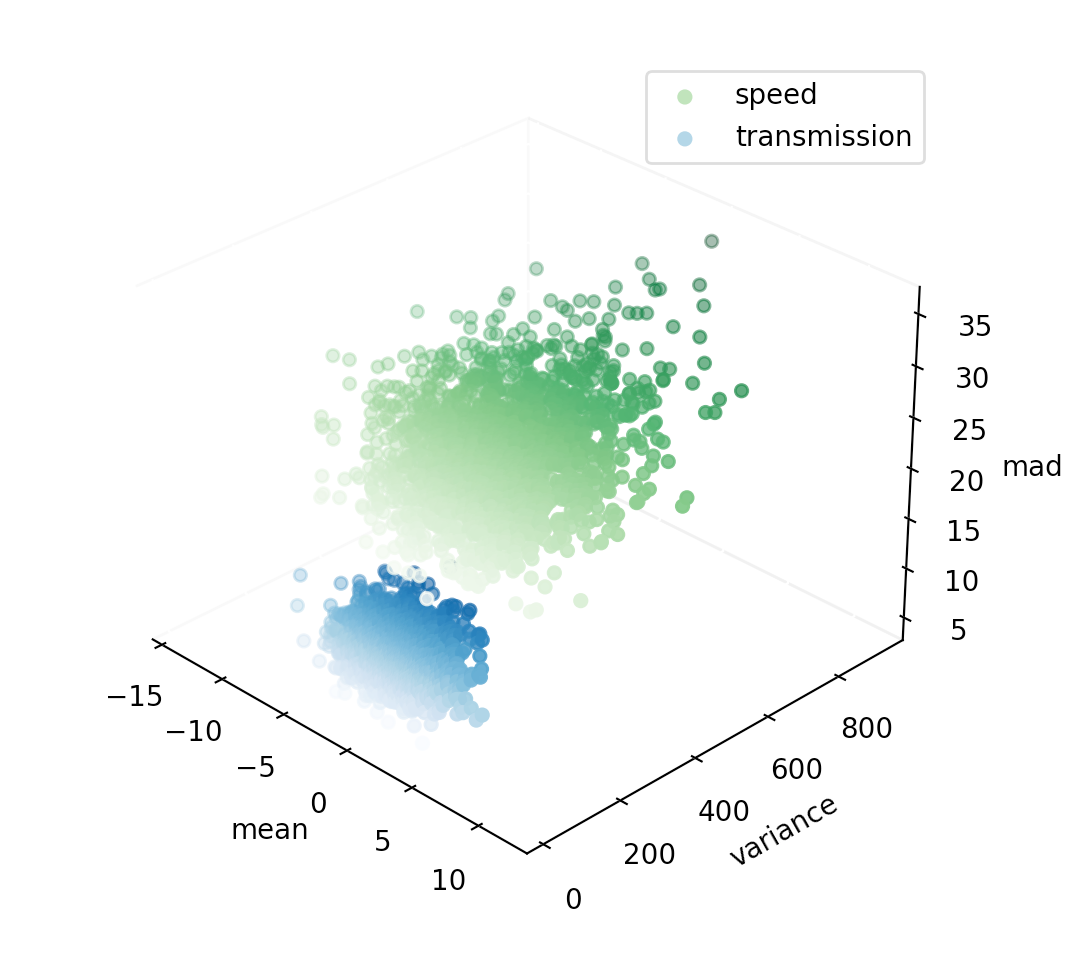
\includegraphics[scale=0.6]{fingerprint.png}
    \centering
    \caption{Esistenza del fingerprint per il modello in Figura \ref{fig:1}.}
    \label{fig:3}
\end{figure}

\begin{table}
    \begin{center}
        \begin{tabular}{|c|c|c|}
            \hline
            \textbf{Dimensione Chunk / Sensore} & \textbf{1} & \textbf{2} \\
            \hline
            5 & 0.879 & 0.772 \\
            \hline
            10 & 0.946 & 0.909 \\
            \hline
            15 & 0.960 & 0.945 \\
            \hline
            20 & 0.978 & 0.977 \\
            \hline
            25 & 0.992 & 0.988 \\
            \hline
            30 & 0.996 & 0.992 \\
            \hline
            35 & 1.000 & 0.995 \\
            \hline
            40 & 0.997 & 1.000 \\
            \hline
            45 & 1.000 & 1.000 \\
            \hline
            50 & 1.000 & 0.993 \\
            \hline
            55 & 1.000 & 1.000 \\
            \hline
        \end{tabular}
    \end{center}
    \caption{Dimensione dei chunk differenti e accuratezza del classificatore per il modello di un'automobile a cambio automatico.}
    \label{tab:2}
    \begin{center}
        \begin{tabular}{|c|c|c|c|}
            \hline
            \textbf{Dimensione Chunk / Sensore} & \textbf{1} & \textbf{2} & \textbf{3} \\
            \hline
            5 & 0.785 & 0.561 & 0.748 \\
            \hline
            10 & 0.850 & 0.723 & 0.906 \\
            \hline
            15 & 0.882 & 0.793 & 0.963 \\
            \hline
            20 & 0.910 & 0.855 & 0.979 \\
            \hline
            25 & 0.911 & 0.894 & 0.990 \\
            \hline
            30 & 0.940 & 0.930 & 0.995 \\
            \hline
            35 & 0.958 & 0.930 & 0.996 \\
            \hline
            40 & 0.969 & 0.946 & 0.998 \\
            \hline
            45 & 0.976 & 0.957 & 1.000 \\
            \hline
            50 & 0.980 & 0.969 & 1.000 \\
            \hline
            55 & 0.984 & 0.984 & 1.000 \\
            \hline
            60 & 0.991 & 0.985 & 1.000 \\
            \hline
            65 & 0.986 & 0.980 & 0.998 \\
            \hline
            70 & 0.991 & 0.983 & 0.998 \\
            \hline
            75 & 0.993 & 0.983 & 1.000 \\
            \hline
            80 & 0.998 & 0.993 & 1.000 \\
            \hline
            85 & 0.995 & 1.000 & 1.000 \\
            \hline
            90 & 0.997 & 0.995 & 1.000 \\
            \hline
            95 & 1.000 & 0.997 & 1.000 \\
            \hline
            100 & 0.997 & 0.991 & 1.000 \\
            \hline
        \end{tabular}
    \end{center}
    \caption{Dimensione dei chunk differenti e accuratezza del classificatore per il modello del controllo automatico del clima di un'automobile.}
    \label{tab:3}
\end{table}

Si vuole ora provare alcuni dei punti anticipati nella Sezione \ref{sec:1}.

\begin{table}
    \begin{center}
        \resizebox{\textwidth}{!}{
        \begin{tabular}{|c|c|}
            \hline
            \RomanNumeralCaps{1} Modello & \RomanNumeralCaps{2} Modello \\
            \hline
            \begin{tabular}{|c|c|c|c|c|c|}
                \textbf{Sensore} & 1 & 2 \\
                \hline
                \textbf{Varianza} & 390 & 100 \\
                \hline
                \textbf{(1 - RMSE)*100} & 83.5\% & 92.0\% \\
            \end{tabular} &
            \begin{tabular}{|c|c|c|c|c|c|}
                \textbf{Sensore} & 1 & 2 & 3 \\
                \hline
                \textbf{Varianza} & 9.2 & 4.2 & 1 \\
                \hline
                \textbf{(1 - RMSE)*100} & 96.4\% & 97.2\% & 99.0\% \\
            \end{tabular} \\
            \hline
        \end{tabular}}
    \end{center}
    \caption{Valori della varianza delle distribuzioni associate ai sensori dei due modelli considerati.}
    \label{tab:6}
\end{table}

Alla luce di quanto detto nella Sezione \ref{sec:1}, per quanto riguarda l'introduzione del rumore gaussiano nei sensori, 
sono state trovate empiricamente le varianze delle distrubizioni tale che valga l'Equazione \ref{eq:7}.
Nella Tabella \ref{tab:6} possiamo vedere i valori per entrambi i modelli.

Nella Figura \ref{fig:3} vedere invece la rappresentazione grafica delle feature statistiche dei vettori dei residui dei due sensori che appartengono al modello in Figura \ref{fig:1}.
\`E facile in questo modo intuire significato del fingerprint, questo ci d\`a un'idea di come il profilo del rumore sia una peculiarit\`a di ogni sensore. Nell'esempio proposto vengono utilizzate tre feature, nello specifico media, varianza e deviazione media assoluta.

Come gi\`a detto in precedenza, per catturare le giuste dinamiche del sistema, vi \`e la necessit\`a di suddividere il dataset in blocchi, e questi non devono avere una dimensione tale da non allungare eccessivamente l'intervallo di tempo che deve passare affinch\'e un attacco venga identificato.
Nel caso del primo modello, il modello SVM viene allenato e validato con dataset composti da feature estratte da chunk che hanno una dimensione variabile e crescente tra un'esecuzione e la successiva. La dimensione dei chunk va da un minimo di 5 fino ad un massimo di 55 misurazioni, con un incremento di 5.
Come si pu\`o vedere dalla Tabella \ref{tab:2} l'accuratezza del classificatore converge verso valori molto vicini ad 1 per chunk di dimensioni maggiore di 25.
Un valore ragionevole potrebbe essere uno tra 25 e 30 in quanto hanno un buonissimo livello di accuratezza ma mantengono una dimensione abbastanza ridotta.
La scelta che \`e stata fatta \`e quella di prendere come dimensione dei blocchi 25, in quanto il modello ha un sample time di $\frac{1}{25}$ secondi e questo permetterebbe di estrarre le feature dal chunk ogni secondo.
Se fosse stata scelta una dimensione di 30 avremmo ottenuto risultati poco differenti.

Nel caso del secondo modello, il modello SVM viene allenato e validato con una dimensione dei chunk che va 5 a 100, con un incremento di 5.
I risultati sperimentali sono mostrati nella Tabella \ref{tab:3} e si pu\`o notare che il classificatore raggiunge un'accuratezza per chunk con una dimensione di 80.
Dato che il sample time del modello \`e di 1 secondo, significa che per poter estrarre le feature dai chunk bisogna attendere 80 secondi.

\begin{table}
    \begin{center}
    \resizebox{\textwidth}{!}{
    \begin{tabular}{|c|c|c|c|c|c|c|c|c|c|c|c|c|c|c|}
        \hline
        \textbf{Split} & 2 & 3 & 4 & 5 & 6 & 7 & 8 & 9 & 10 & 11 & 12 & 13 & 14 & 15 \\
        \hline
        \textbf{Accuratezza} & 0.989 & 0.989 & 0.990 & 0.990 & 0.990 & 0.990 & 0.990 & 0.990 & 0.990 & 0.990 & 0.991 & 0.990 & 0.990 & 0.990 \\
        \hline
    \end{tabular}}
    \end{center}   
    \caption{Risultati, relativi al primo modello, della k-fold cross validation per diversi valori di k, con dimensione dei chunk uguale a 25.} 
    \label{tab:4}
    \begin{center}
    \resizebox{\textwidth}{!}{
    \begin{tabular}{|c|c|c|c|c|c|c|c|c|c|c|c|c|c|c|}
        \hline
        \textbf{Split} & 2 & 3 & 4 & 5 & 6 & 7 & 8 & 9 & 10 & 11 & 12 & 13 & 14 & 15 \\
        \hline
        \textbf{Accuratezza} & 0.987 & 0.988 & 0.988 & 0.987 & 0.987 & 0.988 & 0.988 & 0.988 & 0.988 & 0.988 & 0.988 & 0.988 & 0.988 & 0.988 \\
        \hline
    \end{tabular}}
    \end{center}
    \caption{Risultati, relativi al secondo modello, della k-fold cross validation per diversi valori di k, con dimensione dei chunk uguale a 80.}
    \label{tab:5}
\end{table}

Ora, con l'obiettivo di mostrare il comportamento del classificatore al variare della dimensione del dataset si valutano i risultati  forniti dalla cross validation.
Entrambi i modelli vengono simulati per un determinato tempo per permettere la raccolta dei dati. Anche in questa situazione bisogna trovare un giusto compromesso in quanto 
si cerca di raggiungere tutti gli stati del sistema affinché la probabilit\`a che durante il periodo di vita del sistema (in cui si potrebbero verificare attacchi) ci siano falsi positivi (stati non raggiunti durante la simulazione raggiunti poi durante il normale funzionamento del sistema) sia il pi\`u bassa possibile.

Le simulazioni hanno una durata di 24 ore e 12 ore, rispettivamente per il primo e il secondo modello.
I risultati della cross validation, per differenti valori di k, vengono mostrati nella Tabella \ref{tab:4} per il primo modello e nella Tabella \ref{tab:5} per il secondo.
Si pu\`o notare che il classificatore \`e robusto e mostra che non \`e importante quale range delle serie temporali vengono utilizzate per il trainign e il testing .

% \section{Valutazione computazionale} % probabilmente da rimuovere
% describe here experiments aimed at evaluating computational performance (e.g., CPU usage, RMA usage, etc)

\section{Valutazione tecnica}
% describe here experiments aimed at evaluating your tools wrt their intended use.
% For example, software to detect adversarial attacks will be evaluated here showing how good (or bad) it is in detecting attcks.

In questo capitolo verr\`a presa in considerazione una classe di attacchi ai sensori e la risposta dell'algoritmo di rilevamento.

L'attacco ai sensori viene pensato come un introduzione di rumore gaussiano nelle misurazioni dei sensori. Dato che nell'attuale implementazione viene gi\`a introdotto del rumore gaussiano, come discusso nel Capitolo \ref{chap:4}, un attacco pu\`o essere visto come una variazione (in eccesso) della varianza

\begin{table}
    \begin{center}
        \begin{tabular}{|c|c|c|c|c|}
            \hline
            \textbf{\% varianza / \% chunk} & \textbf{25\%} & \textbf{50\%} & \textbf{75\%} & \textbf{100\%} \\
            \hline
            \begin{tabular}{|c|}
                Sensore \\
                \hline
                \textbf{5\%} \\
                \hline
                \textbf{10\%} \\
                \hline
                \textbf{15\%} \\
                \hline
                \textbf{20\%} \\
            \end{tabular} &
            \begin{tabular}{|c|c|}
                I & II \\
                \hline
                53.2 & 55.8 \\
                \hline
                53.2 & 55.8 \\
                \hline
                53.2 & 55.8 \\
                \hline
                53.2 & 55.8 \\
            \end{tabular}
            \hline
        \end{tabular}
    \end{center}
\end{table}


\begin{sidewaysfigure}[b]
    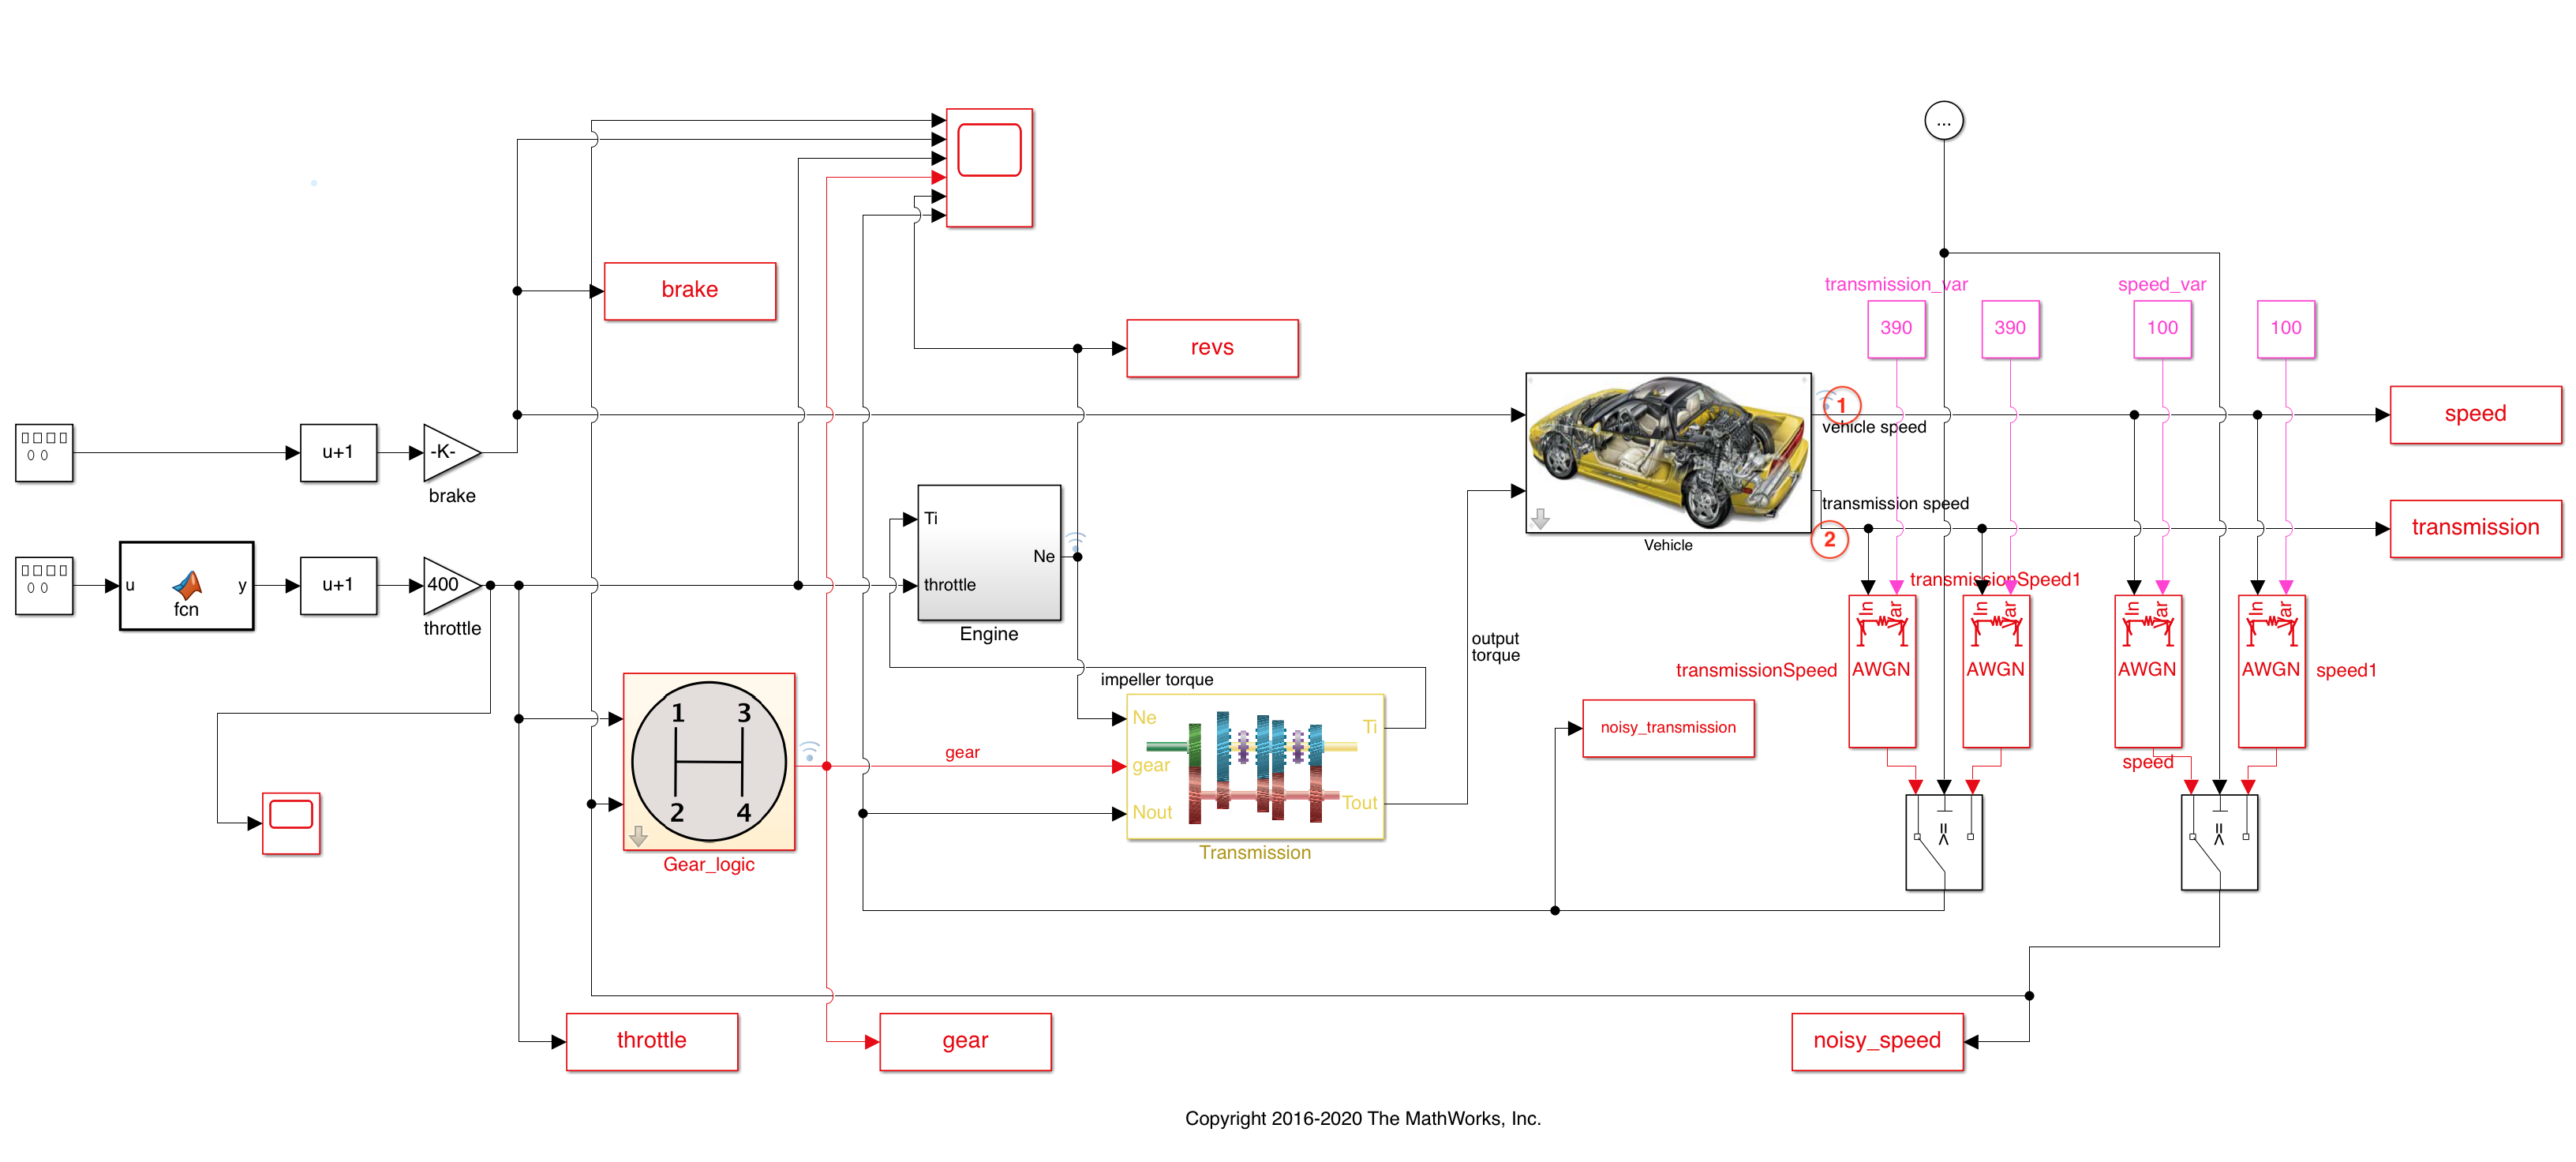
\includegraphics[scale=0.38]{car.png}
    \centering
    \caption{Modello Simulink di un'automobile a trasmissione automatica.}
    \label{fig:1}
\end{sidewaysfigure}

\begin{sidewaysfigure}[b]
    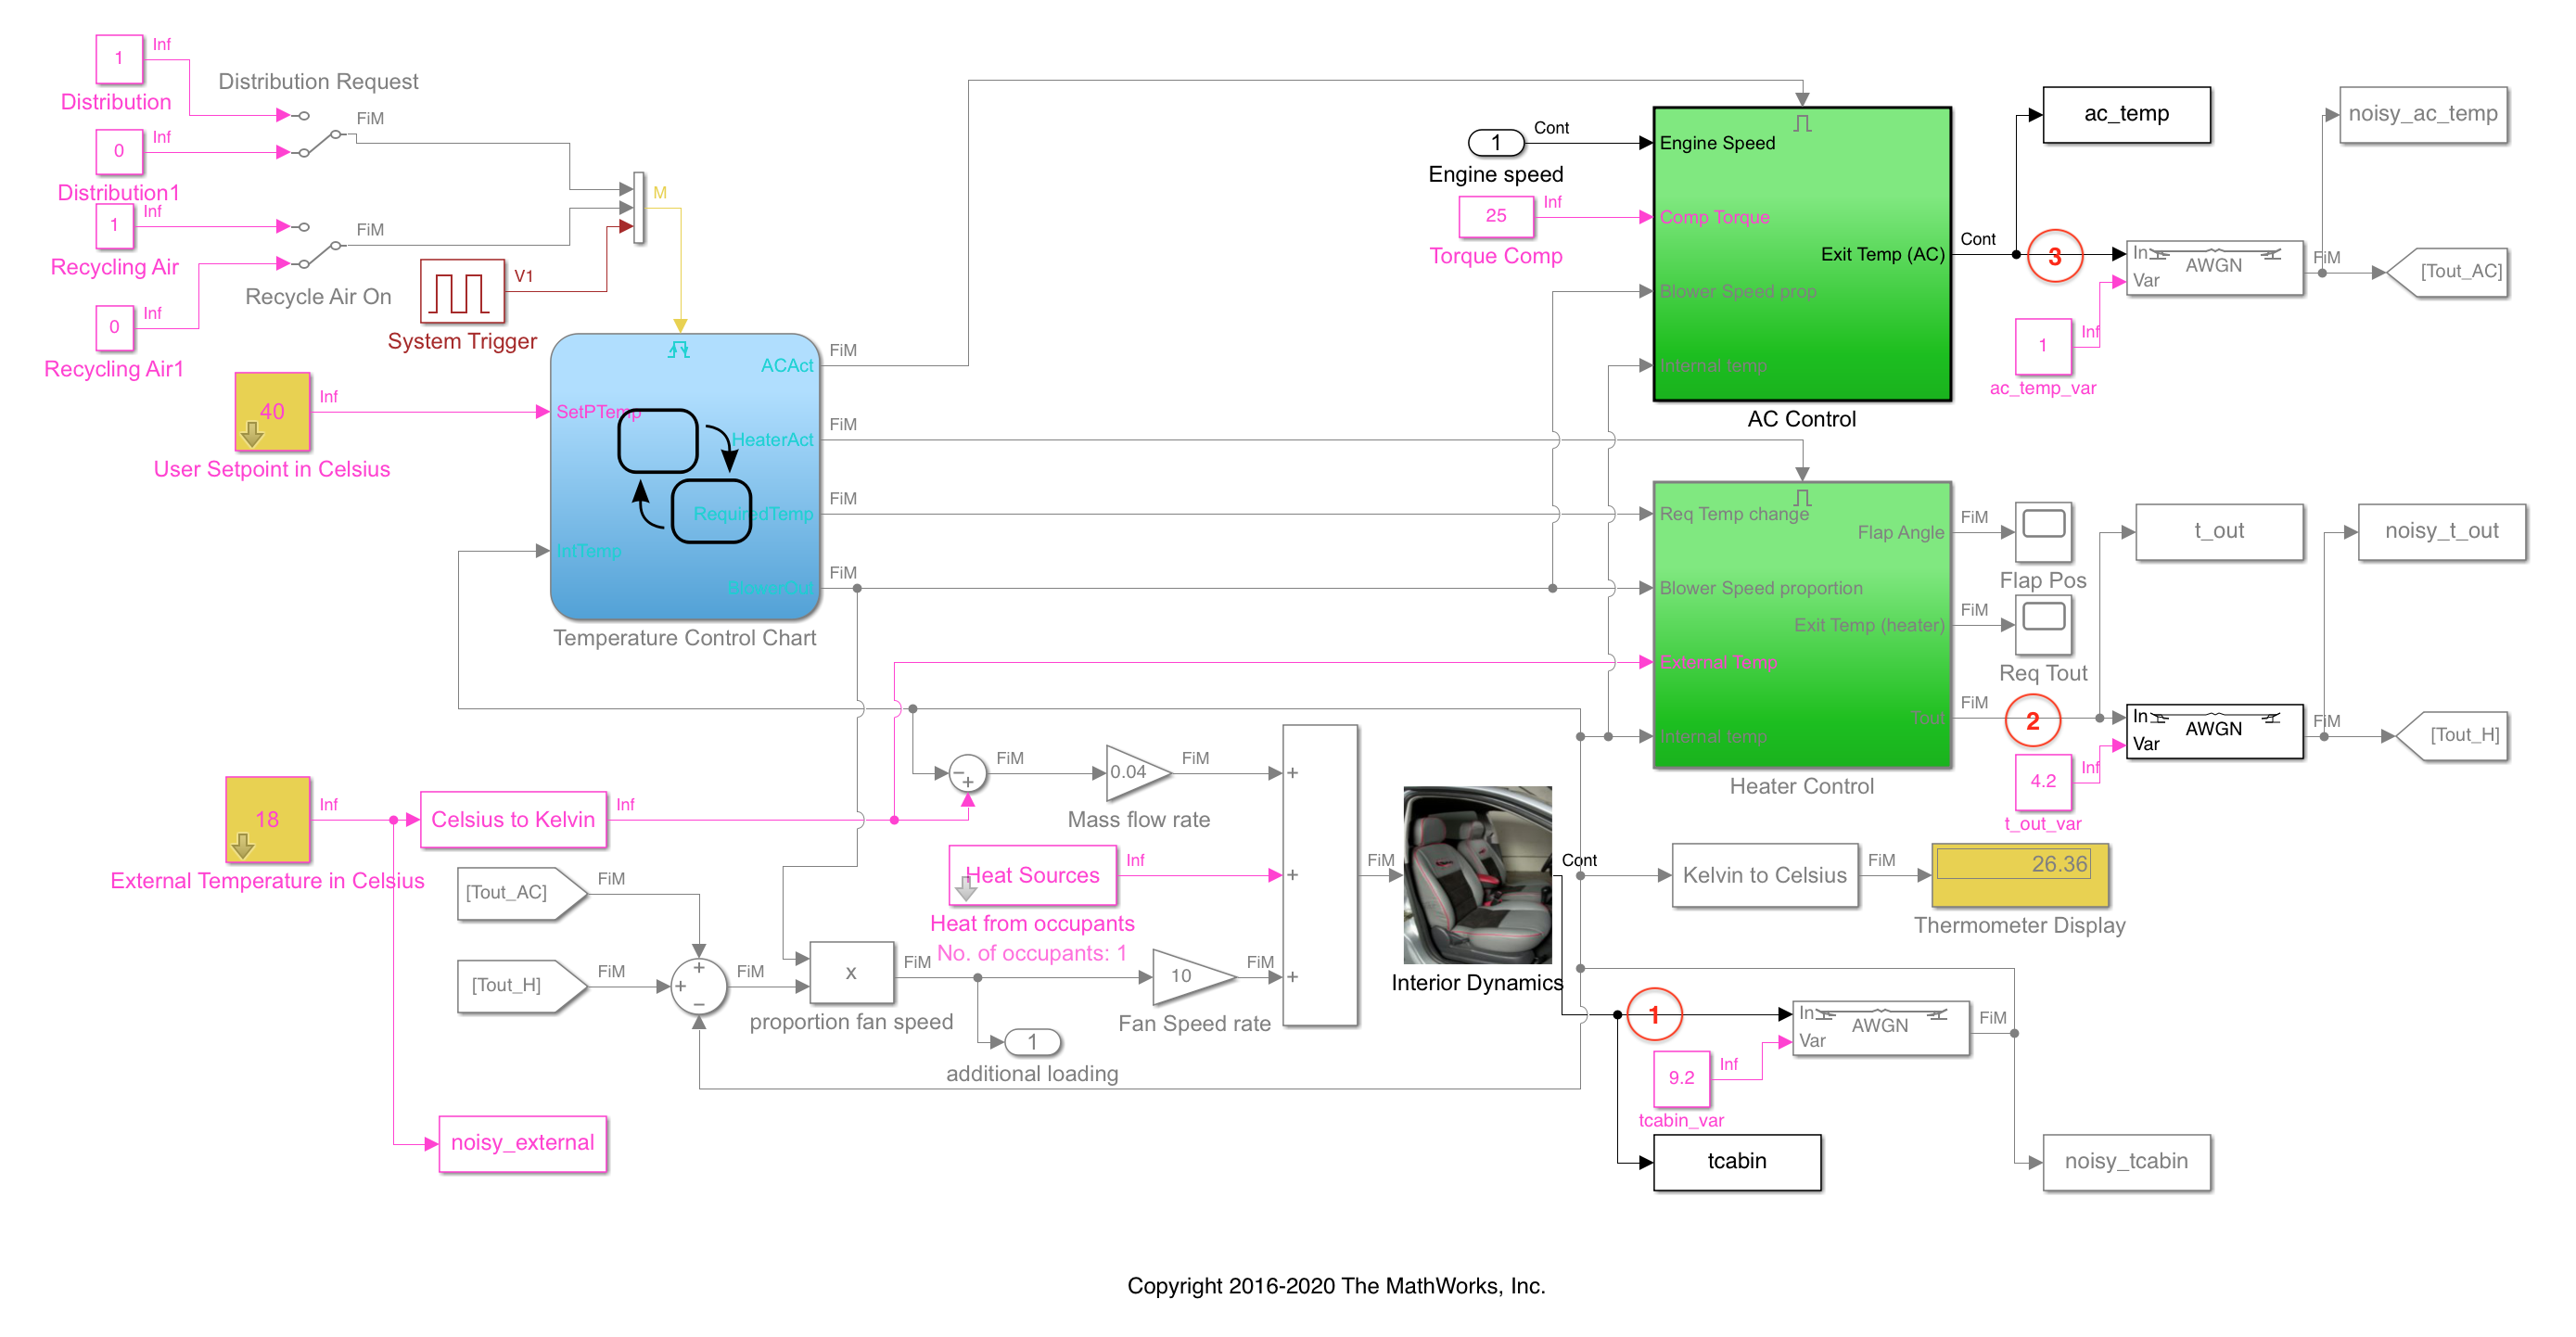
\includegraphics[scale=0.45]{climate.png}
    \centering
    \caption{Modello Simulink di un sistema di controllo automatico del clima dell'ambiente interno di un'autovettura.}
    \label{fig:2}
\end{sidewaysfigure}

\chapter{Conclusioni}
% Sum up what you did and outline some possible future developments.

\backmatter
% Inserire qui referenze e citazioni

\end{document}